\PassOptionsToPackage{utf8}{inputenc}
\documentclass{bioinfo}

\usepackage{makecell}

\usepackage{floatrow}

\usepackage{comment}

\usepackage{siunitx}

%TODO FIX THIS
% singlelinecheck=false puts subcaptions on the left
%\usepackage[singlelinecheck=false]{subcaption}
\usepackage{graphicx}
\usepackage[caption=false]{subfig}
\floatsetup[figure]{subcapbesideposition=top}
%TODO FIX THIS

\usepackage{amsthm}
\theoremstyle{definition}
\newtheorem{definition}{Definition}[section]
\newtheorem{theorem}{Theorem}[section]
\newtheorem{corollary}{Corollary}[theorem]
\newtheorem{lemma}[theorem]{Lemma}

\usepackage{amsfonts}
\usepackage{booktabs}

\usepackage{algorithm2e}
\usepackage[usenames,dvipsnames]{xcolor}
\SetAlgoLined
\usepackage{bm}

% we squeeze our figures even more together
\captionsetup{belowskip=-2pt}

\SetAlgoLined
\SetKwProg{MyStruct}{Struct}{ contains}{end}

\newcommand{\vocab}{\textbf}
\newcommand{\red}[1]{{\textcolor{Red}{#1}}}
\newcommand{\FIXME}[1]{\red{[FIXME: #1]}}

\usepackage{orcidlink}
\hypersetup{hidelinks}
\usepackage{appendix}
\newcommand{\description}{}
\usepackage[inline]{enumitem}

% table stuff
\usepackage{amsfonts}
\usepackage{booktabs}
\usepackage{siunitx}
\newcommand{\ra}[1]{\renewcommand{\arraystretch}{#1}}
\usepackage{stfloats}
\usepackage{hyperref}
%\floatstyle{plaintop}
%\restylefloat{table}

% supplement stuff
\newcommand{\beginsupplement}{%
	\setcounter{table}{0}
	\renewcommand{\thetable}{S\arabic{table}}%
	\setcounter{figure}{0}
	\renewcommand{\thefigure}{S\arabic{figure}}%
}

\def\labelitemi{--}

\copyrightyear{2024} \pubyear{XXXX}

\access{Advance Access Publication Date: Day Month Year}
\appnotes{Genome Analysis}

\begin{document}
    \firstpage{1}

    \subtitle{Genome Analysis}

    \title[\red{Cluster-efficient} pangenome graph construction with nf-core/pangenome]{\red{Cluster-efficient} pangenome graph construction with nf-core/pangenome}
    %\title[Genome-guided pangenome graph layouts via Stochastic Gradient Descent]{Genome-guided pangenome graph layouts via Stochastic Gradient Descent}
	%\title[Sequence-guided pangenome graph layouts via Stochastic Gradient Descent]{Sequence-guided pangenome graph layouts via Stochastic Gradient Descent}
    %\title[Genome-guided pangenome graph layouts]{Genome-guided pangenome graph layouts}
	%\title[Sequence-guided pangenome graph layouts]{Sequence-guided pangenome graph layouts}
    
	\author[Heumos \textit{et~al}.]{
        Simon~Heumos\,$^{\orcidlink{0000-0003-3326-817X}1,2,3,4,*}$,
        Michael~L.~Heuer\,$^{\orcidlink{0000-0002-9052-6000}5}$,
        Friederike~Hanssen\,$^{\orcidlink{0009-0001-9875-5262}1,2,3,4}$,
        Lukas~Heumos\,$^{\orcidlink{0000-0002-8937-3457}6,7,8}$,
        Andrea~Guarracino\,$^{\orcidlink{0000-0001-9744-131X}9,10,}$,
        Peter~Heringer\,$^{\orcidlink{0009-0005-5985-2317}1,2,3,4}$,
        Philipp~Ehmele\,$^{\orcidlink{0000-0001-5945-7839}6}$,
        Pjotr Prins\,$^{\orcidlink{0000-0002-8021-9162}9}$,
        Erik~Garrison\,$^{\orcidlink{0000-0003-3821-631X}9}$,
        Sven Nahnsen\,$^{\orcidlink{0000-0002-4375-0691}1,2,3,4,*}$
    }

    \address{
	$^1$Quantitative Biology Center (QBiC) Tübingen, University of Tübingen, Tübingen, Germany \\ 
	$^2$Biomedical Data Science, Dept. of Computer Science, University of Tübingen, Tübingen, Germany \\ 
	$^3$M3 Research Center, University Hospital Tübingen, Tübingen, Germany \\ 
	$^4$Institute for Bioinformatics and Medical Informatics (IBMI), Eberhard-Karls University of Tübingen, Tübingen, Germany \\ 
	$^5$University of California, Berkeley, Berkeley, 94720, California, USA \\
	$^6$Institute of Computational Biology, Department of Computational Health, Helmholtz Munich, Germany \\ 
	$^7$Comprehensive Pneumology Center with the CPC-M bioArchive, Helmholtz Zentrum Munich, Member of the German Center for Lung Research (DZL), Munich, Germany \\ 
	$^8$TUM School of Life Sciences Weihenstephan, Technical University of Munich, Freising, Germany \\
	$^{9}$Department of Genetics, Genomics and Informatics, University of Tennessee Health Science Center, 71 S Manassas St, Memphis, 38163, Tennessee, USA \\ 
	$^{10}$Human Technopole, Viale Rita Levi-Montalcini 1, 20157, Milan, Italy \\
    }

    \corresp{
        $^\ast$To whom correspondence should be addressed. \\
    }

    \history{Received on XXXXX; revised on XXXXX; accepted on XXXXX}

    \editor{Associate Editor: XXXXXXX}

	\abstract{
	\textbf{Motivation:}
	Pangenome graphs offer a comprehensive way of capturing genomic variability across multiple genomes. 
	However, current construction methods often introduce biases, excluding complex sequences or relying on references. 
	The PanGenome Graph Builder (PGGB) addresses these issues. 
	To date, though, there is no state-of-the-art pipeline allowing for easy deployment, efficient and dynamic use of available resources, and scalable usage at the same time.
	%Yet, its bash implementation hinders deployment, resource optimization, and scalability for large-scale graph construction. 
	\\
	\textbf{Results:}
	To overcome these limitations, we present \textit{nf-core/pangenome}, a reference-unbiased approach implemented in Nextflow following nf-core's best practices. 
	Leveraging biocontainers ensures portability and seamless deployment in HPC environments. 
	%SN: in any compute infrastructure, such as HPCs or clouds
	Unlike PGGB, nf-core/pangenome distributes alignments across cluster nodes, enabling scalability. 
	Demonstrating its efficiency, we constructed pangenome graphs for 1000 human chromosome 19 haplotypes and 2146 \textit{E. coli} sequences, achieving a two to threefold speedup compared to PGGB without increasing greenhouse gas emissions. \\
	\textbf{Availability:}
	nf-core/pangenome is released under the MIT open-source license, available on \href{https://github.com/nf-core/pangenome}{GitHub} and \href{https://zenodo.org/doi/10.5281/zenodo.8202636}{Zenodo}, with documentation accessible at \href{https://nf-co.re/pangenome/1.1.2/docs/usage}{https://nf-co.re/pangenome/1.1.2/docs/usage}. \\
	\textbf{Contact:} \href{simon.heumos@qbic.uni-tuebingen.de}{simon.heumos@qbic.uni-tuebingen.de}, \href{sven.nahnsen@qbic.uni-tuebingen.de}{sven.nahnsen@qbic.uni-tuebingen.de} \\
%	Pangenome graphs can encode the entire genomic variability between multiple genomes. Current pangenome graph construction methods exclude complex sequences or are reference-based, leading to reference, order, or orientation bias. This was addressed by the PanGenome Graph Builder (PGGB) pipeline. 
%	However, PGGB’s bash implementation limits its ease of deployment, optimal use of compute resources, and cluster scalability, making it impractical to build very large pangenome graphs.
%	\\
%	\textbf{Results:}
%	We implemented \textit{nf-core/pangenome}, a reference-unbiased approach to construct pangenome graphs. 
%	Mirroring PGGB, it iteratively refines an all-to-all whole-genome alignment graph that allows to explore sequence conservation and variation, infer phylogeny, and identify recombination events. 
%	nf-core/pangenome is implemented in Nextflow and follows the nf-core best practice development guidelines. 
%	Providing all software dependencies in biocontainers makes the pipeline portable and easy to install on high-performance computing environments. 
%	In contrast to PGGB, this allows nf-core/pangenome to distribute the quadratically complex all-to-all base-level alignments across nodes of a cluster. 
%	%Evaluating 1024 \textit{E. coli} haplotypes, the time spent on base-pair level alignments is reduced linearly with an increase in alignment problem chunks. 
%	To demonstrate the scalability of nf-core/pangenome, we built pangenome graphs of 1000 chromosome 19 human haplotypes, and of 2146 \textit{E. coli} sequences. nf-core/pangenome was two to three times faster compared to PGGB while not increasing the greenhouse gas emissions.
%	\\
%	\textbf{Availability:}
%	nf-core/pangenome is published as free software under the MIT open-source license. Source code can be downloaded from \url{https://github.com/nf-core/pangenome} and the documentation is accessible at \url{https://nf-co.re/pangenome/1.1.2/docs/usage}. 
%	Each release is archived on Zenodo \texttt{\href{https://zenodo.org/doi/10.5281/zenodo.8202636}{10.5281/zenodo.8202636}}. \\
%	\textbf{Contact:} \href{simon.heumos@qbic.uni-tuebingen.de}{simon.heumos@qbic.uni-tuebingen.de}, \href{sven.nahnsen@qbic.uni-tuebingen.de}{sven.nahnsen@qbic.uni-tuebingen.de} \\
	%\textbf{Supplementary information:} Supplementary data are available online. %at \textit{Bioinformatics} online.
	}
	
	\maketitle
	\vspace{-0.5cm}
	\section{Introduction}
	The availability of high-quality collections of population-wide whole-genome assemblies \citep{Liao2023, Kang2023, Weller2023, Zhou2022, Liu2020, Leonard2022} offers new opportunities to study sequence evolution and variation within and between genomic populations. 
	A challenge is simultaneously representing and analyzing hundreds to thousands of genomes at a gigabase scale. 
	One solution here is a pangenome. It models a population's entire set of genomic sequences \citep{Ballouz2019}. 
	In contrast to reference-based genomic approaches, which relate sequences to a linear genome, pangenomics relates each new sequence to all the others represented in the pangenome \citep{CompPan2016, Eizenga_2020, Sherman_2020} minimizing reference-bias. 
	Pangenomes can be described as sequence graphs which store DNA sequences in nodes with edges connecting the nodes as they occur in the individual sequences \citep{Hein1989}. 
	Genomes are encoded as paths traversing the nodes \citep{Garrison:2018}.
	
	Current pangenome graph construction methods exclude complex sequences or are reference-biased \citep{Chin2023, Minkin2016}.
	%, are tree-guided, or reference-based \citep{Li:2020, Hickey2023} leading to reference, order, or orientation bias. 
	%Although whole genome scaling approaches for unbiased pangenome graph construction \citep{Chin2023, Minkin2016} exist, their reliance on k-mer-based data structures often leads to unwanted complexity for downstream analysis. 
	One recent approach that overcomes such limitations is the PanGenome Graph Builder (PGGB) pipeline \citep{Garrison2023}. 
	PGGB iteratively refines an all-to-all whole-genome alignment graph that lets us explore sequence conservation and variation, infer phylogeny, and identify recombination events. 
	PGGB was already extensively evaluated \citep{Garrison2023, Andreace2023} and applied to build the first draft human pangenome reference \citep{Liao2023}.
	However, PGGB is implemented in bash\red{, which (a)} makes it difficult to deploy on HPC systems, (b) does not allow for a fine granular tuning of computing resources for different steps of the pipeline \citep{Sztuka2024}, and (c) limits its cluster scalability because PGGB can only use the resources of one node. These limitations greatly hinder the broad application of large-scale pangenomes.
	%SN: Given the high resource requirements of large-scale pangenomes, %these limitations are significantly limiting broad applications.
	
	To compensate for that, we wrote \textit{nf-core/pangenome}, a reference-unbiased approach to construct pangenome graphs. 
	Mirroring PGGB, nf-core/pangenome is implemented in Nextflow \citep{DiTommaso2017}.
	% and follows the community-curated nf-core \citep{Ewels2020} best practice development guidelines. 
	%Providing all software dependencies in biocontainers \citep{daVeigaLeprevost2017} makes the pipeline portable and easy to install on HPC environments. 
	In contrast to PGGB, nf-core/pangenome can distribute the quadratic all-to-all base-level alignments across nodes of a cluster by splitting the approximate alignments into problems of equal size. 
	We benchmarked the time spent on base-pair level alignments and show that it is reduced linearly with an increase in alignment problem chunks \red{(Suppl. ~\ref{aln_jobs_dist})}. 
	We showcase the workflow’s scalability by applying it to 1000 chromosome 19 human haplotypes, and to 2146 \textit{E. coli} sequences, which were built in less than half the time PGGB required while not increasing the CO2 equivalent (CO2e) emissions.
	\vspace{-0.6cm}
	\section{Material and Methods}
	
	\subsection{Pipeline overview}
	The pipeline’s (Fig. \ref{fig:workflow}) input is a FASTA file compressed with \textit{bgzip} \citep{Li2009} containing the sequences to create the graph. 
	Sequence names should follow the Pangenome Sequence Naming specification (PanSN-spec) \citep{pansn-spec}. 
	The primary output is a pangenome variation graph \citep{Garrison:2018} in the Graphical Fragment Assembly (GFA) format version 1 \citep{GFA}.
	
	\begin{figure*}[]
	\sidesubfloat[First subfigure]{%
	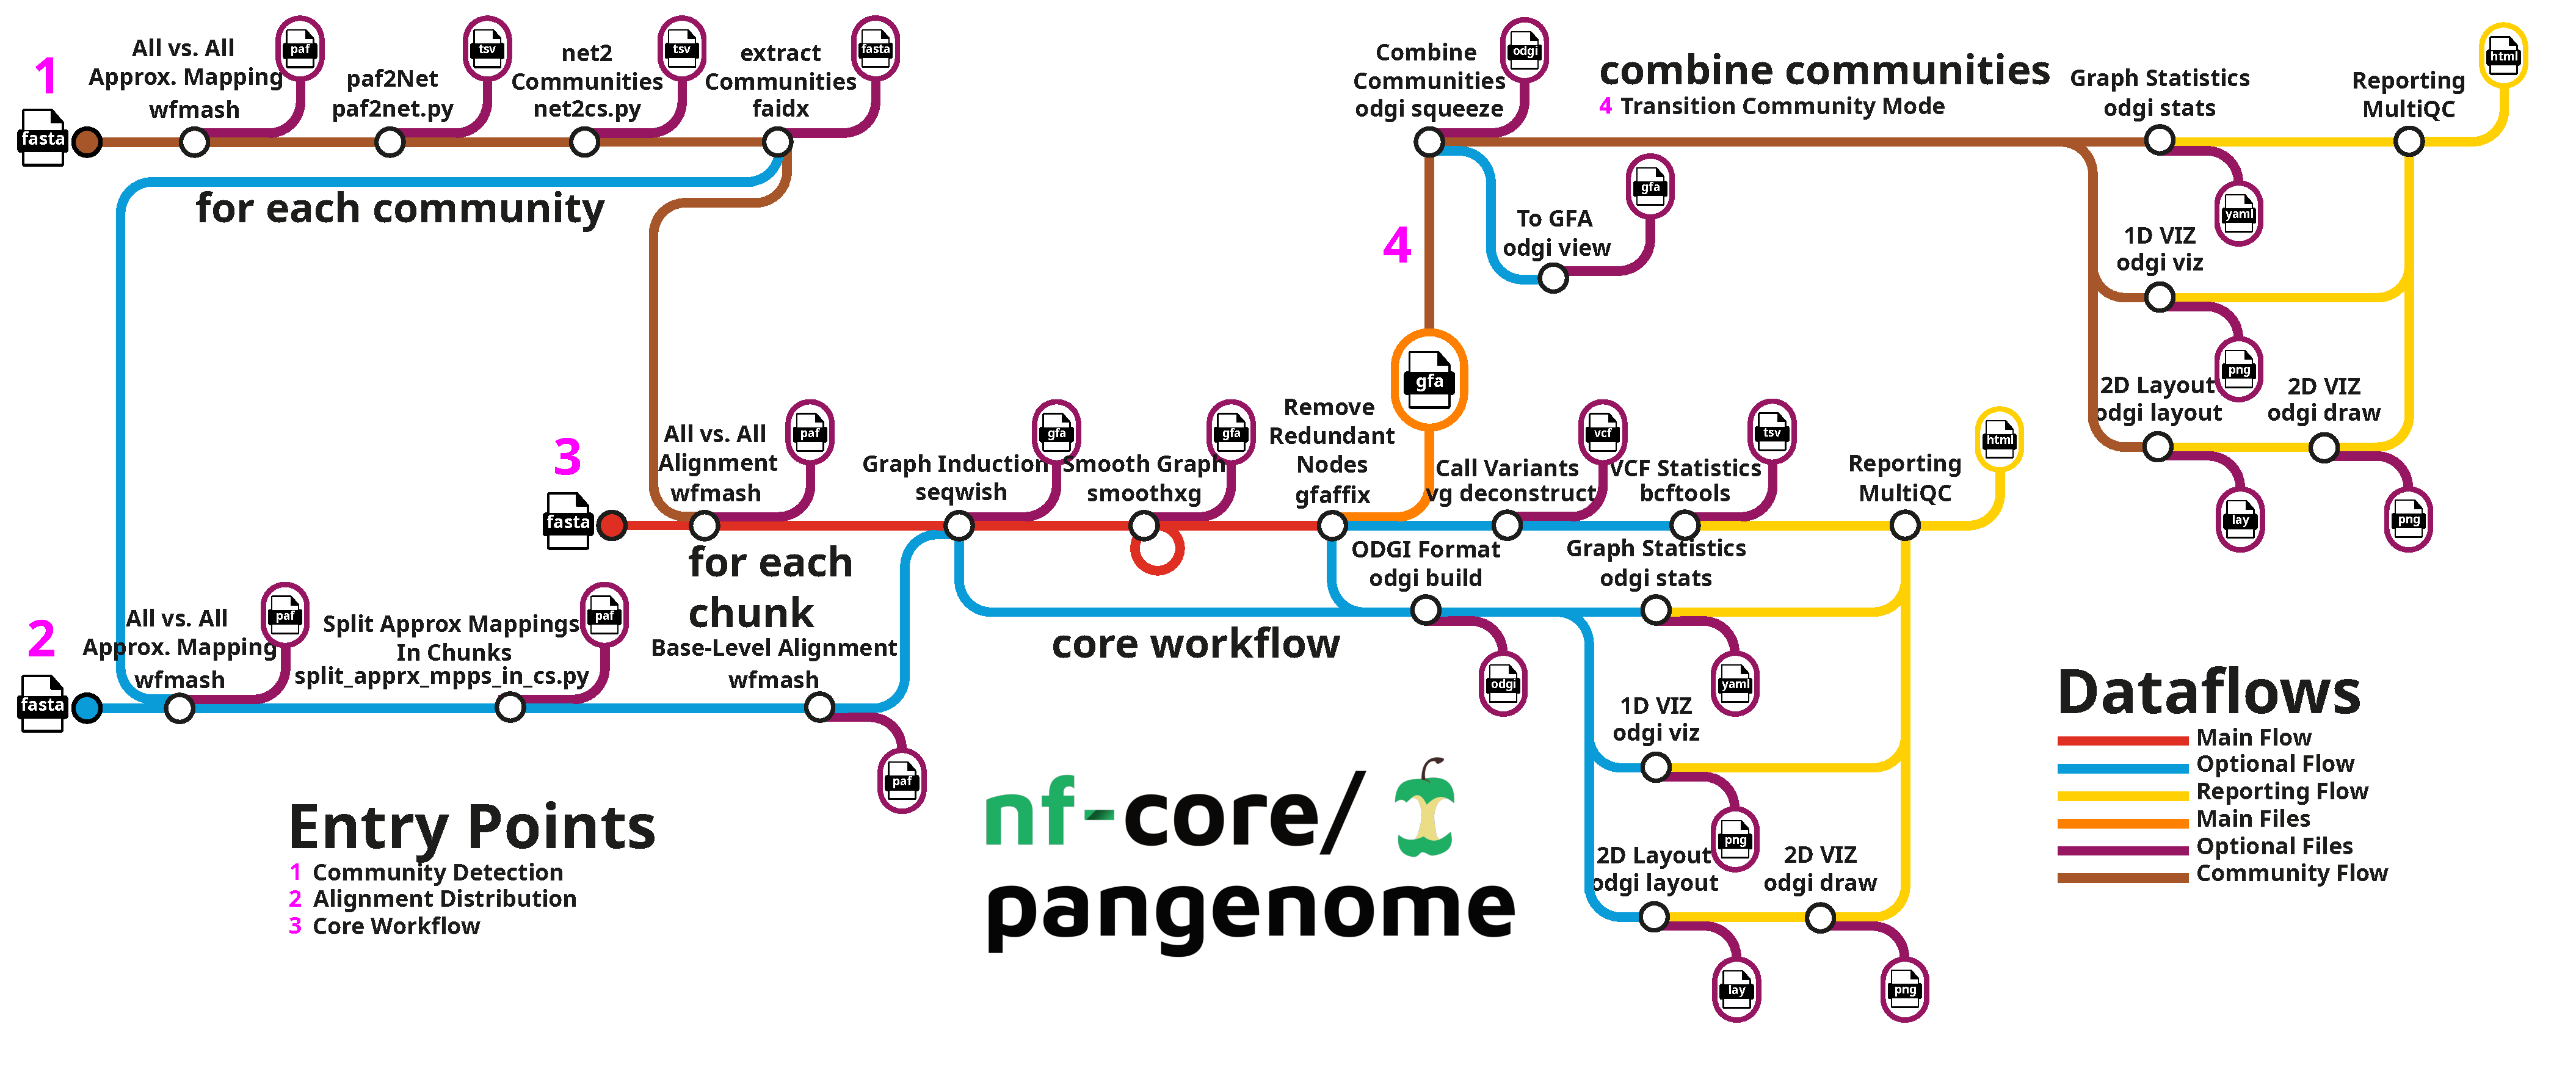
\includegraphics[width=\textwidth]{fig/pangenome_workflow.pdf}
	\label{fig:workflow}
	}
	\vspace{-0.3cm}
	\hfill
	\sidesubfloat[Second subfigure]{%
	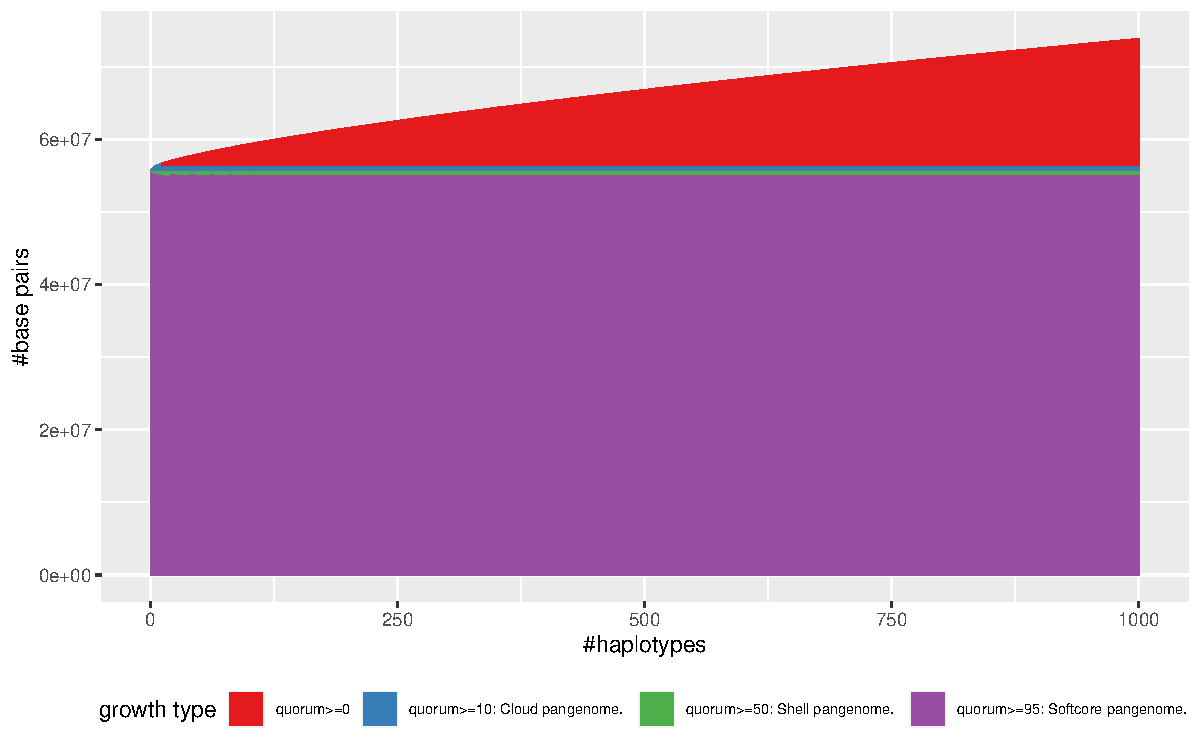
\includegraphics[width=0.45\textwidth]{fig/chr19_histgrowth.pdf}
	\label{fig:hist_chr19}
	}
	\sidesubfloat[Second subfigure]{%
	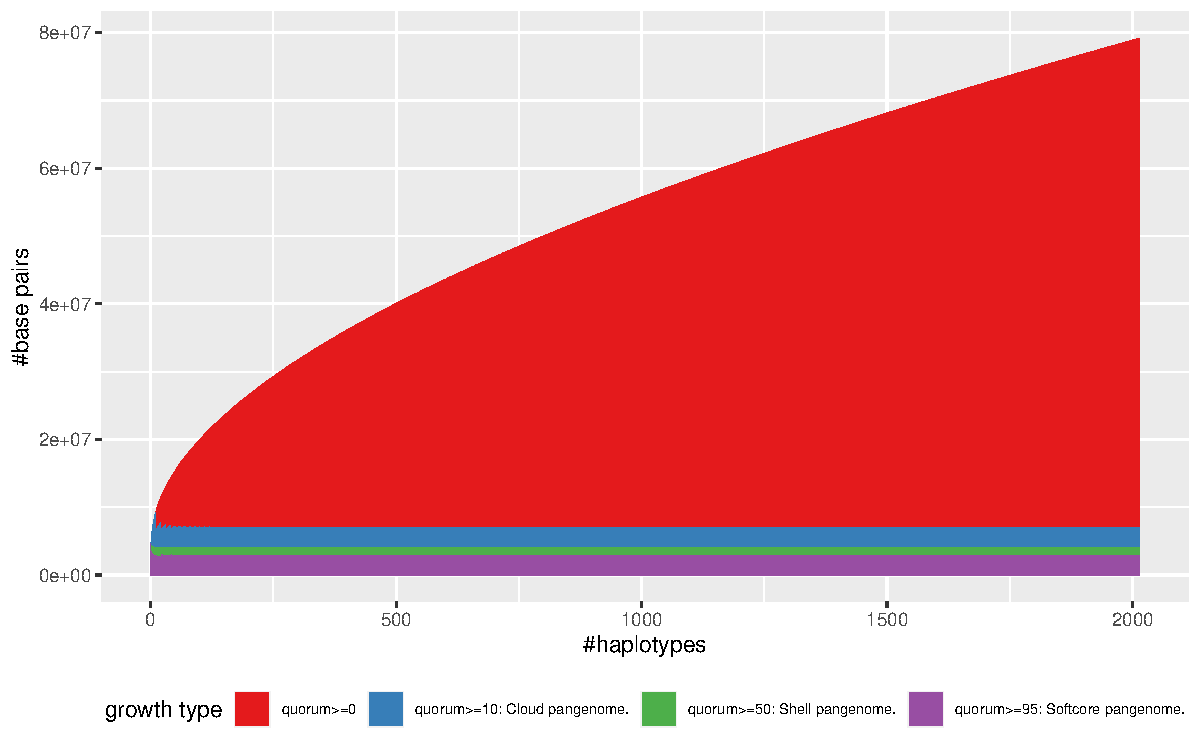
\includegraphics[width=0.45\textwidth]{fig/ecoli2013_histgrowth.pdf}
	\label{fig:hist_ecoli}
	}
	%\sidesubfloat[Second subfigure]{%
	%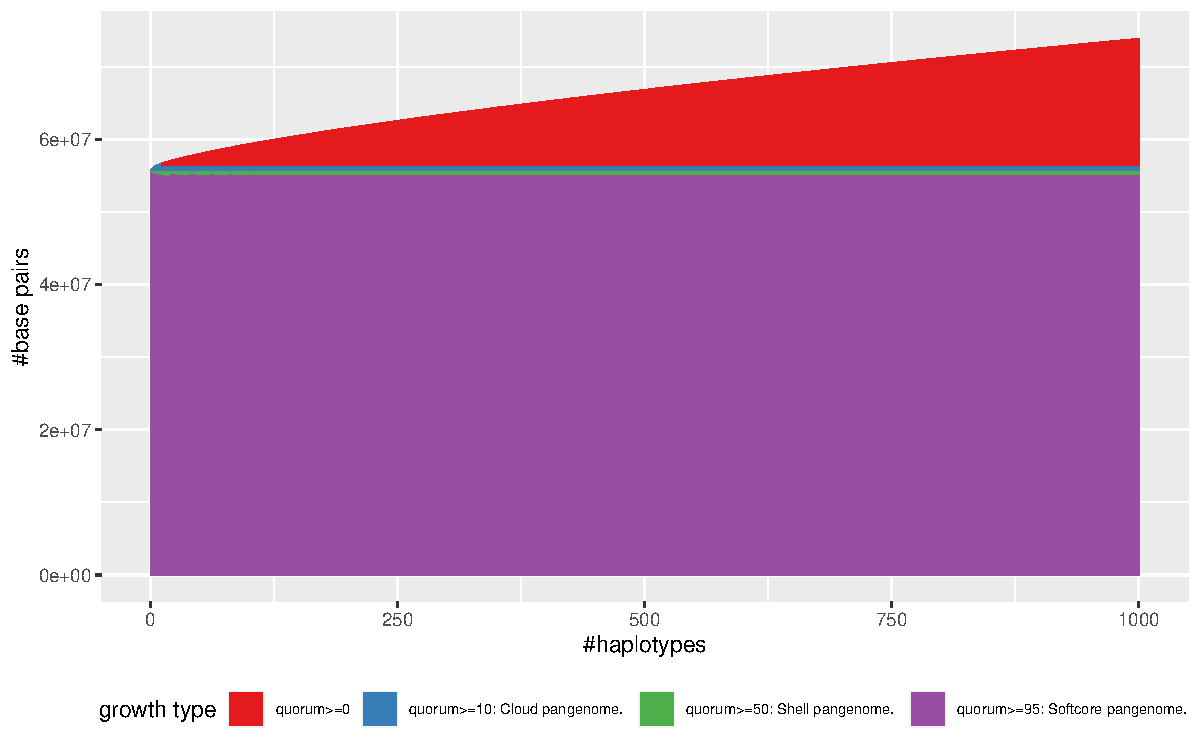
\includegraphics[width=0.3\textwidth]{fig/chr19_histgrowth.pdf}
	%\label{fig:hist_ecoli}
	%}
	\vspace{-0.25cm}
	\caption{\textbf{(a)} Schematic representation of the nf-core/pangenome workflow processes and detailed analysis steps. The input consists of one FASTA file containing all sequences. The pipeline comes with 3 major entry points: \red{(1) Community detection, which identifies clusters of related sequences or regions in the pangenome graph to reveal biologically significant patterns like conserved or divergent areas across genomes~(Supplementary \ref{community}), (2) alignment distribution, and (3)  core workflow.} Optional community detection (1) is performed on the input sequences. If selected, the heavy all-to-all baise-pair level alignments (2) can be split into problems of equal size. nf-core/pangenome’s core workflow (3) is a direct mirror of PGGB. If running in community mode, all communal graphs are combined into one (4) and the subsequent quality control subworkflow is executed. The output is a pangenome graph in GFA format. \textbf{(b) + (c)} Pangenome growth curves of the built pangenome graphs. Growth type is defined as the minimum fraction of haplotypes that must share a graph feature after each time a haplotype is added to the growth histograph. $quorum>=0$: All sequences without any filtering are considered. $quorum>=10$: Sequences traversed by at least 10\% of the haplotypes. $quorum>=50$: Sequences traversed by at least 50\% of haplotypes. $quorum>=95$: Sequences traversed by 95\% of haplotypes. \textbf{(b)} Pangenome growth curve of the chromosome 19 pangenome graph of 1000 haplotypes. \textbf{(c)} Pangenome growth curve of the \textit{E. coli} pangenome graph of 2013 haplotypes.
	}
	\label{fig:panel}
\end{figure*}
\vspace{-0.5cm}

	\subsubsection{Core workflow}
	
	The core workflow of nf-core/pangenome \red{mirrors}\red{ PGGB (Fig. \ref{fig:workflow}) with additional enhancements:} (a) All concurrent processes can be run in parallel. (b) Each process can be given individual computing resources.
	%This results in efficient resource management, especially compared to PGGB, which uses the same resources for all steps of the pipeline. 
	
	\red{The pipeline begins with an all-to-all alignment of the input sequences using the whole-chromosome pairwise sequence aligner WFMASH \citep{wfmash}, avoiding reference, order, or orientation bias, allowing every sequence to serve as a reference.}
	%This avoids reference, order, or orientation bias, and allows each sequence in the pangenome to serve as a reference when exploring related variation. 
	In the pangenome graph induction step SEQWISH \citep{Garrison2022}, an alignment to variation graph inducer, converts the sequence alignments into a variation graph. 
	%SEQWISH can recapture homology relationships that may not be encoded in the initial alignments. 
	%This allows us to randomly sparsify the mappings computed by WFMASH. 
	%The applied heuristic is based on the Erdös-Rényi random graph model \citep{Bollobs2001}. 
	\red{The graph is then simplified using SMOOTHXG \citep{Garrison2023}:}
	A 1-dimensional (1D) graph embedding \citep{Heumos2023} orders the graphs’ nodes to best-match the nucleotide distances of the genomic paths of the graph.
	%This considers the local spurious complexity inherent in the raw pairwise alignments. 
	%If ignored, this could lead to difficulties in downstream processing of the graph.
	%Therefore, SMOOTHXG iteratively applies a local Multiple Sequence Alignment (MSA), partial order alignment (POA) \citep{Lee2002}, to refine and compress the pangenome graph. A 1-dimensional (1D) graph embedding \citep{Heumos2023} gives rise to the regions the kernel is applied to. 
	%After applying the graph embedding algorithm, the graphs’ node order best-matches the nucleotide distances of the genomic paths of the graph. 
	Next, the graph is split into partially overlapping segments. 
	%The sequences of each segment are realigned with POA. 
	The sequences of each segment are realigned with a local Multiple Sequence Alignment (MSA) kernel, partial order alignment (POA) \citep{Lee2002}.
	Afterwards, the segments are laced back together into a variation graph. 
	By default, the SMOOTHXG process is applied 3 times in order to smoothen the edge effects at the boundaries of the segments.
	Finally, we employ GFAFFIX \citep{Liao2023} to systematically condense redundant nodes within the graph.
	%In the final normalization phase, we employ GFAFFIX \citep{Liao2023} to systematically condense redundant nodes within the graph. 
	%Subsequently, the 1D graph embedding algorithm is reapplied to ensure a human-readable representation of the processed data. 
	%For more details about each step, we refer to the original PGGB paper (Garrison et al. 2023).
	
	\red{Graph quality is assessed with ODGI~\citep{Guarracino2022}, which provides statistics and visualizations.} %: Optimized Dynamic Genome/Graph Implementation \citep{Guarracino2022} for understanding pangenome graphs. ODGI reports basic graph statistics and diagnostic 1D and 2D visualizations. 
	%Specifically, ODGI reports basic graph statistics, such as the length, and the number of nucleotides, paths, edges, nodes, and components. ODGI’s human readable 1D and 2D visualizations help to understand if the biology encoded in the graph fits the expectations. 
	%Six different 1D views focus on displaying the relative alignments of the graph’s paths, while the 2D view highlights high-level features such as SVs. 
	%Additionally, the 2D TSV layout of ODGI can be interactively explored in the variation graph visualizers gfaestus (\href{https://github.com/chfi/gfaestus}{https://github.com/chfi/gfaestus}) or waragraph (\href{https://github.com/chfi/waragraph}{https://github.com/chfi/waragraph}). 
	\red{Optionally, variants can be called against any (reference) path(s) in the graph using \textit{vg deconstruct} \citep{Garrison:2018}. 
	Results are summarized in a MultiQC \citep{Ewels_2016} report.} 
	Pipeline implementation details are given in Suppl.~\ref{implementation}.
	
\red{	If desired, the pipeline performs community detection to identify clusters of related sequences in the pangenome graph, revealing biological patterns such as conserved or divergent regions across genomes (Supplementary 5.2), with the core workflow executed for each community in parallel.}
	\vspace{-0.6cm}
	\section{Results}
	
	%\subsection{Alignment jobs distribution evaluation}
	
	%Generating all-vs-all alignments is a computationally quadratic problem. 
	%To evaluate nf-core/pangenome’s alignment jobs scalability (detailed in Suppl. ~\ref{aln_jobs_dist}), we applied it to 1024 \textit{E. coli} genomes with varying numbers of chunks. 
	%nf-core/pangenome’s alignment jobs distribution linearly reduces the time spent on base-pair level alignments with increased chunks.
	%The CO2 consumption is not influenced by the number of chunks (Suppl. Fig.~\ref{fig:emissions}).
	%\vspace{-0.0cm}	
	\subsection{Building a 1000 haplotypes chr19 pangenome graph}
	
	The Human Pangenome Resource Consortium (HPRC) recently built a draft human pangenome reference of 90 haplotypes \citep{Liao2023}. 
	However, haplotype data for thousands of individuals already exists generated by the 1000 Genomes Project (1KGP) \citep{Durbin2010}. 
	As a use case study, we used nf-core/pangenome to build a pangenome graph of 1000 chromosome 19 haplotypes \citep{Kuhnle2020} within 3 days. 
	The CO2e was 22.52 kg. PGGB built the same graph within 7 days. 
	In Fig.~\ref{fig:hist_chr19} the pangenome growth curve generated with PANACUS \citep{Liao2023} shows a growth of the number of nucleotides with an increasing number of haplotypes.
	The size of the softcore pangenome does not change with increasing numbers of haplotypes.
	%One reason for this could be that the input sequences were generated from short read data leaving out complex regions like the centromere.
	
	\subsection{Building a 2146 sequences \textit{E. coli} pangenome graph}
	
	To evaluate the pipeline’s scalability, we built a pangenome graph of 2146 \textit{E. coli} sequences. 
	nf-core/pangenome built the pangenome graph in 10 days, emitting 175.18 kg of CO2e. 
	Due to wall clock time restrictions on our cluster, PGGB was not able to finish the graph construction within 30 days. 
	To build a reasonable pangenome growth curve (Fig.~\ref{fig:hist_ecoli}) we dropped all paths containing “plasmid” (130 in total) in their name. 
	The softcore pangenome of the graph does not change with an increasing number of haplotypes (stable at ~3Mb of sequence), but the general growth curve is steep. 
	%One reason for such a high pangenomic growth is most likely horizontal gene transfer: 
	%Bacteria incorporate genes from each other at different locations in their genome. Other reasons could be sequencing errors or human contamination \citep{Breitwieser2019}.

	\vspace{-0.5cm}
	\section{Discussion}
	
	We implemented nf-core/pangenome, an easy-to-install, portable, and cluster-scalable pipeline for the unbiased construction of pangenome variation graphs.  
    \red{It is the first pangenomic pipeline within the nf-core framework that enables the comparative analysis of gigabase-scale pangenome datasets. 
    While other tools such as Minigraph \citep{Li:2020} or PGR-TK \citep{Chin2023} also address pangenome analysis, nf-core/pangenome uniquely integrates this capability into the standardized nf-core framework, offering compatibility with a wide range of modular workflows and community-developed best practices.}
    
	The pipeline’s core workflow steps were already successfully applied to \textit{Neisseria meningitidis} \citep{Yang2023}, wild grapes \citep{Cochetel2023}, humans \citep{Guarracino2023, Liao2023}, grapevines \citep{Guo2024}, taurines \citep{Milia2024}, and rats \citep{Villani2024} underpinning the community effort to focus on a best-practice workflow to create reference-unbiased and sequence complete pangenome graphs. 
	The modular domain-specific language (DSL) 2 pipeline structure eases the exchange of key processes with alternative tools, the extent of the pipeline with new tools, and the integration of parts of the pipeline with other (sub-)workflows.
	
	We have shown that we are able to perform all-vs-all base pair level alignments of thousands of sequences. 
	When executed on an HPC, nf-core/pangenome’s parallel workflow accelerates graph construction compared to PGGB. 
	PGGB’s inability to assign individual computational resources to each pipeline step leads to the allocation of one whole node of an HPC, despite the fact that some processes can only make use of one thread. 
	This blocks valuable CPU cycles for other users working on the same HPC and ultimately can lead to additional costs.
	%, or, as was shown for \textit{E. coli}, to an inability to finish the graph construction in one go. 
	In contrast, %, utilizing the power of workflow management systems, 
	nf-core/pangenome does not have such limitations: 
	Nextflow’s process management enables the optimal workload of given compute resources which can be especially important when running a pipeline in commercial clouds. %commercial cloud like AWS. 
	%Such savings become increasingly important when one has to iterate the graph construction several times in order to ensure that the built graph best models the biology of the input sequences. 
	%For example, the PGGB HPRC graph construction was iterated 88 times \citep{Liao2023}.
	
	Competing pipelines don’t use any workflow management system to connect their processes \citep{Chin2023}, or their workflow language of choice is e.g. Toil \citep{Vivian2017, Hickey2023} which makes them less user-friendly, less \red{cluster-efficient}, and less portable \citep{Wratten2021}.
	nf-core/pangenome is currently the only pangenomics pipeline that is optionally monitoring its CO2 footprint. 
	The measurements have shown that constructing extensive pangenome graphs, such as the 2146 \textit{E. coli} graph, requires a considerable amount of energy. 
	Therefore, before executing environmentally questionable experiments, we would recommend thoroughly assessing both the rationale and the methodology. 
	%One computationally expensive part is the POA phase of SMOOTHXG. 
	%Adjusting SMOOTHXG with architecture-specific compilation would result in a speedup of approximately 10 times for this specific POA phase. 
	%Progress towards implementing such an enhancement is currently underway. %(\href{https://github.com/pangenome/smoothxg/issues/208}{https://github.com/pangenome/smoothxg/issues/208}).
	
	Although, we expect our pipeline to scale well for future pangenome graph construction challenges, such as for the next HPRC phase which targets \red{350} individuals, there still is potential for further optimization: 
	IMplicit Pangenome Graph (IMPG) (\href{https://github.com/ekg/impg}{https://github.com/ekg/impg}) \red{which is} a tool that extracts homologous loci from all genomes mapped to a specific target region. 
	This would allow us to break the whole genome multiple alignments into smaller pieces, construct a pangenome graph for each piece, and lace these together into a full graph with \href{https://github.com/pangenome/gfalace}{https://github.com/pangenome/gfalace}. 
	%Our first trials 
	%(\href{https://hackmd.io/vh0Ap65uQTm40DdleA-Oow}{https://hackmd.io/vh0Ap65uQTm40DdleA-Oow}) 
	%suggest following this direction.
	
	We anticipate the pipeline, or its parts, will enhance current single linear reference analysis methods to explore whole population variation instead of focusing on one reference only. Looking ahead, pangenome construction pipelines like nf-core/pangenome will play a pivotal role in studying entire populations, single-cell whole genome sequencing analysis, and constructing personalized (medical) pangenome references \citep{Sirn2023}.
	%We believe that the pipeline or parts of it will enhance existing single linear reference analysis methods to explore whole population variation instead of focusing on one reference only. We envision for the future that pangenome construction pipelines, like nf-core/pangenome, will play a pivotal role in studying whole populations, single-cell whole genome sequencing analysis, and, for example, specifically when it comes to the construction of personalized (medical) pangenome references \citep{Sirn2023}. 
	\vspace{-0.6cm}
	\section*{Software and data availability}
	
	Code and links to data resources used to build this manuscript and its figures, can be found in the paper’s public repository: \href{https://github.com/subwaystation/pangenome-paper}{https://github.com/subwaystation/pangenome-paper}.
	\vspace{-0.6cm}
	\section*{Acknowledgments}

	We thank Matthias Seybold from QBiC for maintaining the Core Facility Cluster. 
	We thank Sabrina Krakau from QBiC for giving feedback to the nf-co2footprint plugin section. 
	We are grateful to the nf-core community for their support during the implementation of the pipeline. 
	From the nf-core community, we want to thank Matthias Hörtenhuber, Maxime Garcia, Susanne Jodoin, Julia Mir Petrol, Adam Talbot, and Gisela Gabernet. 
	%We are grateful for extensive support of PANACUS from Daniel Dörr.

	\vspace{-0.6cm}
	
	\section*{Funding}
	
	 S.H. acknowledges funding from the Central Innovation Programme (ZIM) for SMEs of the Federal Ministry for Economic Affairs and Energy of Germany. This work was supported by the BMBF-funded de.NBI Cloud within the German Network for Bioinformatics Infrastructure (de.NBI) (031A532B, 031A533A, 031A533B, 031A534A, 031A535A, 031A537A, 031A537B, 031A537C, 031A537D, 031A538A). A.G. acknowledges support from the Human Technopole. S.N. acknowledges support from iFIT funded by the Deutsche Forschungsgemeinschaft (DFG, German Research Foundation) under Germany’s Excellence Strategy—EXC 2180—390900677 and CMFI under EXC 2124–390838134. 
     \red{We gratefully acknowledge support from NIH/NIDA U01DA047638 (E.G.), NIH/NIGMS R01GM123489 (E.G., P.P.), and NSF PPoSS Award \#2118709 (E.G., P.P.), and the CITG (E.G.).}
	 
	\vspace{-0.6cm}
	
	\section*{Competing interests}
	Author L.H. is employed by LaminLabs.
	
	\vspace{-0.6cm}
	
%	\section*{Author contributions}
%	
%	\emph{Project conception}: Simon Heumos, Michael L. Heuer, Sven Nahnsen \\ 
%	\emph{Software development}: Simon Heumos, Michael L. Heuer, Lukas Heumos, Andrea Guarracino, Peter Heringer, Philipp Ehmele \\ 
%	\emph{Experimental design}: Simon Heumos \\ 
%	\emph{Experimental execution}: Simon Heumos \\ 
%	\emph{Paper writing}: Simon Heumos \\ 
%	\emph{Paper editing}: Simon Heumos, Friederike Hanssen, Lukas Heumos, Andrea Guarracino, Sven Nahnsen \\ 
%	\emph{Documentation}: Simon Heumos \\ 
%	\emph{Software testing}: Simon Heumos, Michael L. Heuer, Friederike Hanssen \\ 
%	\emph{Software review}: Friederike Hanssen \\ 
%	\emph{Project guidance}: Pjotr Prins, Erik Garrison, Sven Nahnsen \\ 
%	\emph{HPC resources}: Sven Nahnsen \\
		
	\bibliographystyle{natbib}
	
	\bibliography{document}
	
	\clearpage
	\setcounter{page}{1}
	
	\beginsupplement
	
	\section{Supplement}
	
	\subsection{Implementation}
	\label{implementation}
	
	nf-core/pangenome is written in Nextflow using its latest domain-specific language (DSL) 2 syntax which facilitates a modular pipeline structure. 
	Each software tool is an individual process that is implemented in its own module (\href{https://nf-co.re/docs/contributing/modules}{https://nf-co.re/docs/contributing/modules}). 
	Processes are concatenated into subworkflows (\href{https://nf-co.re/docs/contributing/subworkflows}{https://nf-co.re/docs/contributing/\\subworkflows}). 
	Developed with the nf-core framework, the pipeline follows a set of best-practice guidelines ensuring high-quality development, maintenance, and testing standards. Specifically, we provide community support via a dedicated Slack channel (\href{https://nfcore.slack.com/channels/pangenome}{https://nfcore.slack.com/channels/pangenome}), GitHub issues, and detailed documentation (\href{https://nf-co.re/pangenome/1.1.2/docs/usage}{https://nf-co.re/pangenome/\\1.1.2/docs/usage}).
	Versioning and portability are enabled through (a) semantic versioning (\href{https://semver.org/}{https://semver.org/}) of the pipeline via tagged releases on GitHub, (b) packaging software dependencies in archivable containers so that the software compute environment is the same across different systems, and (c) summarizing software versions and parameters in the MultiQC report of the pipeline. 
	nf-core/ pangenome uses biocontainers to facilitate portability across different computing resources like HPC clusters, cloud platforms, or local machines. 
	Code changes are evaluated with GitHub Actions’ continuous integration (CI) using a pipeline-specific small test data set. 
	For each new pipeline release, a full-size test is run on Amazon Web Services (AWS) validating the code integrity and cloud compatibility of real-world data sets.
	Specifically, a pangenome graph is created from the 8 Saccharomyces cerevisiae strains of the Yeast Population Reference Panel (YPRP) (Yue and Liti 2018). 
	The results of such a run are available on the nf-core webpage (\href{https://nf-co.re/pangenome/1.1.2/results/pangenome/results-0e8a38734ea3c0397f94416a0146a2972fe2db8b}{https://nf-co.re/pangenome/1.1.2/results/pangenome/results-0e8a38734ea3c0397f9\\4416a0146a2972fe2db8b}). 
	Because we implemented our processes using DSL2 nf-core/modules (\href{https://github.com/nf-core/modules}{https://github.com/nf-core/modules}), they can be distributed easily to other users to share commonly used processes or subworkflows across pipelines. This boosts the reuse of existing work done by the community to be integrated into future pipelines.
	
	\subsection{Chromosome community detection}
	\label{community}
	
	\red{Chromosome community detection involves identifying clusters of closely related sequences or genomic regions within the pangenome graph. These communities represent areas of high similarity or shared sequence variants across multiple genomes. Detecting such communities allows researchers to focus on biologically meaningful patterns, such as conserved or highly divergent regions, which are crucial for understanding genetic diversity, evolutionary relationships, and genotype-phenotype associations.}
	
	\red{For example, eukaryotic genomes are typically organized into chromosomes, and this organization is considered during graph construction in community detection mode. Chromosome groupings from the input sequence are examined, and homologies detected in the all-to-all WFMASH mapping step are passed through the Leiden clustering algorithm \citep{Traag2019}, where the edge weight is calculated as $mapped\_length * mapped\_identity$. The nf-core/pangenome core workflow is then executed in parallel for each of the resulting communities. The communal graphs are subsequently merged into a single graph, followed by a final round of quality control (see Fig~\ref{fig:workflow}, brown tubes).}
	
	\red{This approach works effectively for large input sequences with a mapping length filter greater than 1 Mb, as demonstrated by \cite{Guarracino2023} when exploring recombination between heterologous human acrocentric chromosomes.}
	
	\subsection{Compute environment}
	
	We applied the nf-core/pangenome pipeline v1.1.2 to various inputs evaluating both the scalability of the all-vs-all alignment step as well as the pipeline as a whole. 
	We used Nextflow version 23.10.1.5891 and Singularity version 3.8.7-1.el8 for each pipeline run. 
	Experiments were conducted on our core facility cluster (CFC) with 24 Regular nodes (32 cores / 64 threads with two AMD EPYC 7343 processors with 512 GB RAM and 2 TB scratch space) and 4 HighMem nodes (64 cores / 128 threads with two AMD EPYC 7513 processors with 2048 GB RAM and 4TB scratch space). 
	Each Nextflow process was given at most 64 threads. This ensures a fair run time comparison with PGGB v0.5.4 which was always executed on one Regular node via Slurm.
	
	\subsection{Estimation of the carbon footprint of pipeline runs}
	
	We also estimated the carbon dioxide equivalent (CO2e) emissions of each nf-core/pangenome pipeline run using the nf-co2footprint Nextflow plugin (\href{https://github.com/nextflow-io/nf-co2footprint}{https://github.com/nextflow-io/nf-co2footprint}) v1.0.0-beta. 
	Using the Nextflow resource usage metrics and information about the power consumption of the compute system, the plugin first estimates the energy consumption for each pipeline task. 
	It then uses the consumed energy's location-specific carbon intensity to estimate the respective CO2e emission.
	The calculations are based on the carbon footprint computation method developed in the Green Algorithms project (\href{www.green-algorithms.org}{www.green-algorithms.org}) \citep{Lannelongue2021}.
	
	\subsection{Alignment jobs distribution}
	\label{aln_jobs_dist}

	The computationally heavy all versus all base-pair level alignments can be distributed across nodes of a cluster: 
	First, WFMASH is run in mapping mode (WFMASH MAP), finding all sequence homologies using approximate alignments. 
	The resulting Pairwise mApping Format (PAF) file is split into chunks of equal problem size. 
	The number of chunks is manually selected. 
	The value can be guided by the number and size of the input sequences, and by the available hardware. 
	Assuming the number of chunks equals the number of nodes on a cluster, then potentially each base-pair level alignment (WFMASH ALIGN) can be run in parallel on each node  (Fig. \ref{fig:workflow}, cyan tubes). 
	All resulting PAFs are then forwarded to the pipeline’s core workflow which is continued at the SEQWISH process.
	
	\begin{figure}[htpb]
	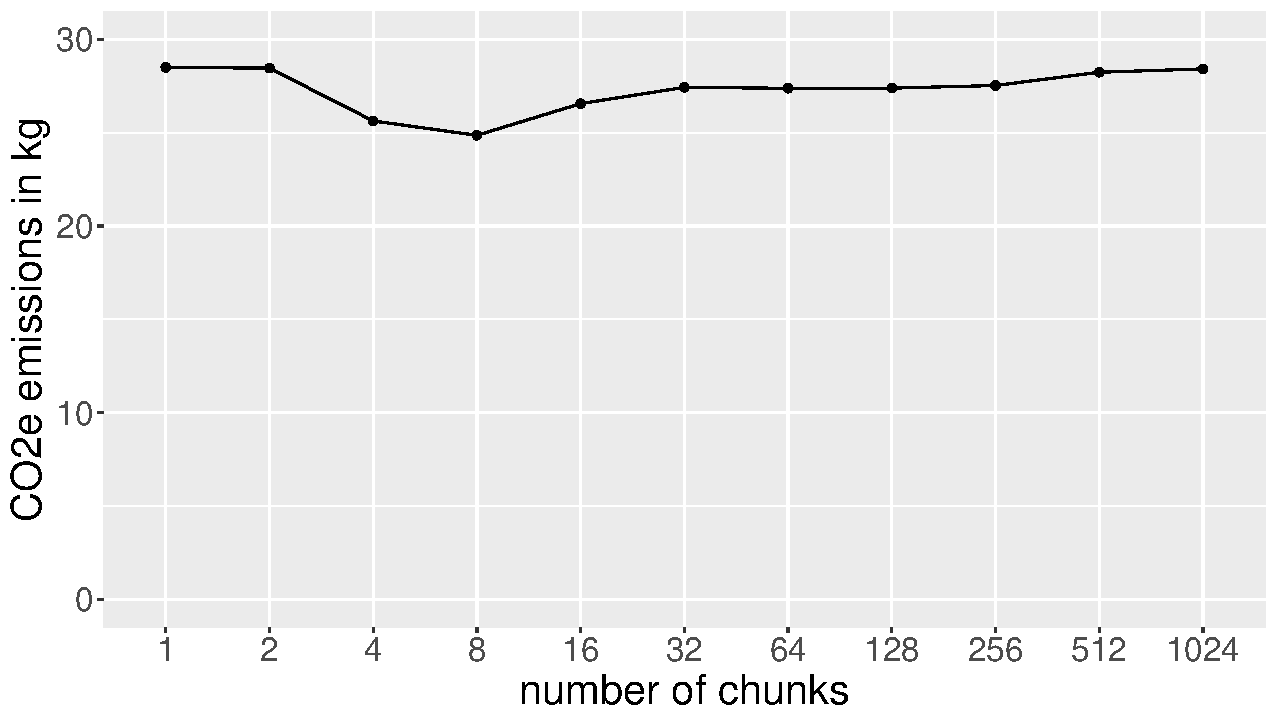
\includegraphics[width=\textwidth]{fig/by_chunks_ALIGN_emissions.pdf}
	\label{fig:emissions}
	\caption{Base-pair level alignment evaluation. CO2e emissions are stable across varying numbers of chunks.
	}
\end{figure}
	
	\subsection{1KGP chromosome 19 data set}
	
	The FASTA of the chromosome 19 data set was downloaded in December 2023 from \href{http://dolomit.cs.tu-dortmund.de/chr19.1000.fa.xz}{http://dolomit.cs.tu-dortmund.de/chr19.1000.fa.xz}. The data set is described in \citep{Kuhnle2020}. Statistics of the built pangenome graph can be seen in Supplementary Fig. ~\ref{fig:chr19_multiqc}. The initial graph contains over 97\% of Ns. We applied \textit{odgi crush} (odgi version 0.8.6), which crushes consecutive Ns of all nodes containing Ns into just one N per node, to the 1KGP chromosome 19 pangenome graph. This brings down the number of Ns from over 3B to exactly 6000 (Suppl. Fig.~\ref{fig:chr19_multiqc}). 
	The 2D visualization (Suppl. Fig.~\ref{fig:chr19_2D}) is perfectly linear without any large SVs present hinting that only short-read data was used to create the haplotype sequences.
	In contrast, the 2D layout of the HPRC PGGB chromosome 19 pangenome graph \citep{Heumos2023} clearly presents SVs, especially in the centromere's location. Investigating these complex regions of a human chromosome is only possible when using long-read assemblies for graph construction.
	
	\begin{figure*}[]
	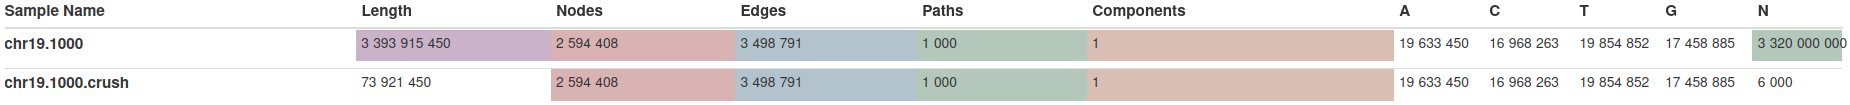
\includegraphics[width=\textwidth]{fig/chr19_multiqc.png}
	\label{fig:chr19_multiqc}
	\caption{Screenshot of the output of ODGI’s MultiQC module displaying the vital graph statistics calculated by odgi stats of the 1000 Genomes Project 1000 haplotypes chromosome 19 pangenome graphs. In the crushed graph consecutive Ns of all nodes containing Ns were merged into just one N per node. A: Number of adenine bases in the graph. C: Number of cytosine bases in the graph. T: Number of thymine bases in the graph. G: Number of guanine bases in the graph. N: Number of bases with unknown base identity.
	}
\end{figure*}
	\begin{figure*}[]
	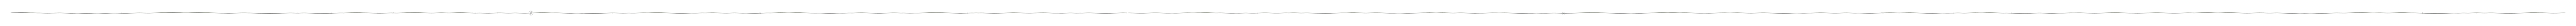
\includegraphics[width=\linewidth]{fig/chr19_2D.png}
	\label{fig:chr19_2D}
	\caption{\textit{odgi draw} 2D layout displaying the graph topology of the crushed 1KGP pangenome graph. Structural variation would appear as bubbles. 
	}
\end{figure*}
	
	\subsection{\textit{E.coli} data set}
	
	The 2146 full length E. coli sequences originate from Genbank \citep{Sayers2021} and were downloaded ~18 months ago. The initial pangenome consisted of 2 graphical components (Suppl. Fig.~\ref{fig:ecoli_multiqc}). This means that no strong homologies were found in some sequences. There can be many reasons for additional graph components: (a) The chosen sequence identity during the WFMASH mapping was not low enough. Although we went for a low 90\% sequence identity (as was done by \cite{Garrison2023}), we still observe this additional graph component, so its sequence must be quite dissimilar to all other sequences. (b) There is human contamination in the bacterial sequences \citep{Breitwieser2019}. (c) Some sequences from GenBank may be of a low quality or were misassembled. We then used odgi explode to extract the largest graphical component, applied \textit{odgi crush} and dropped all paths containing “plasmid” in their path name with \textit{odgi paths}. This left us with one component and 2013 paths.
	In the 2D visualization, we observe a highly connected graph (Suppl. Fig.~\ref{fig:ecoli_2D}). All the reasons mentioned above, but especially horizontal gene transfer could explain this phenomenon. Therefore, there are a lot of edge crossings in the pangenome graph. The long stretches is dangling sequence. We speculate that here the 88 thousand Ns could play role.
	
	\begin{figure*}[]
	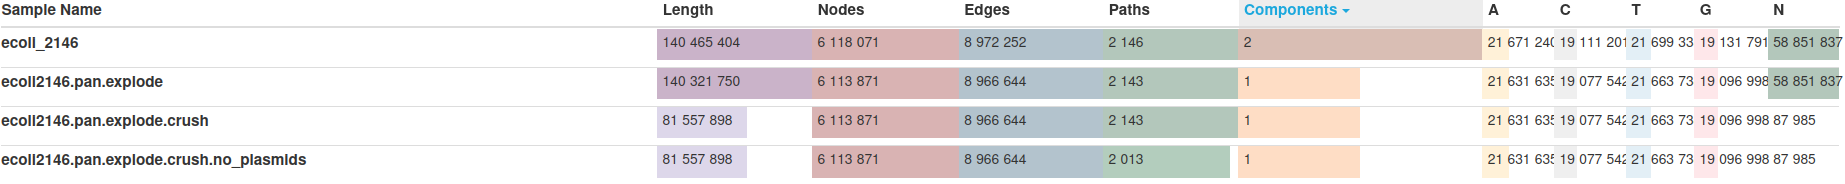
\includegraphics[width=\textwidth]{fig/ecoli_multiqc.png}
	\label{fig:ecoli_multiqc}
	\caption{Excerpt of the 2146 sequences E. coli pangenome graph’s MultiQC report. Displayed are vital graph statistics by MultiQC’s ODGI module. A: Number of adenine bases in the graph. C: Number of cytosine bases in the graph. T: Number of thymine bases in the graph. G: Number of guanine bases in the graph. N: Number of bases with unknown base identity.
	}
\end{figure*}
	\begin{figure*}[]
	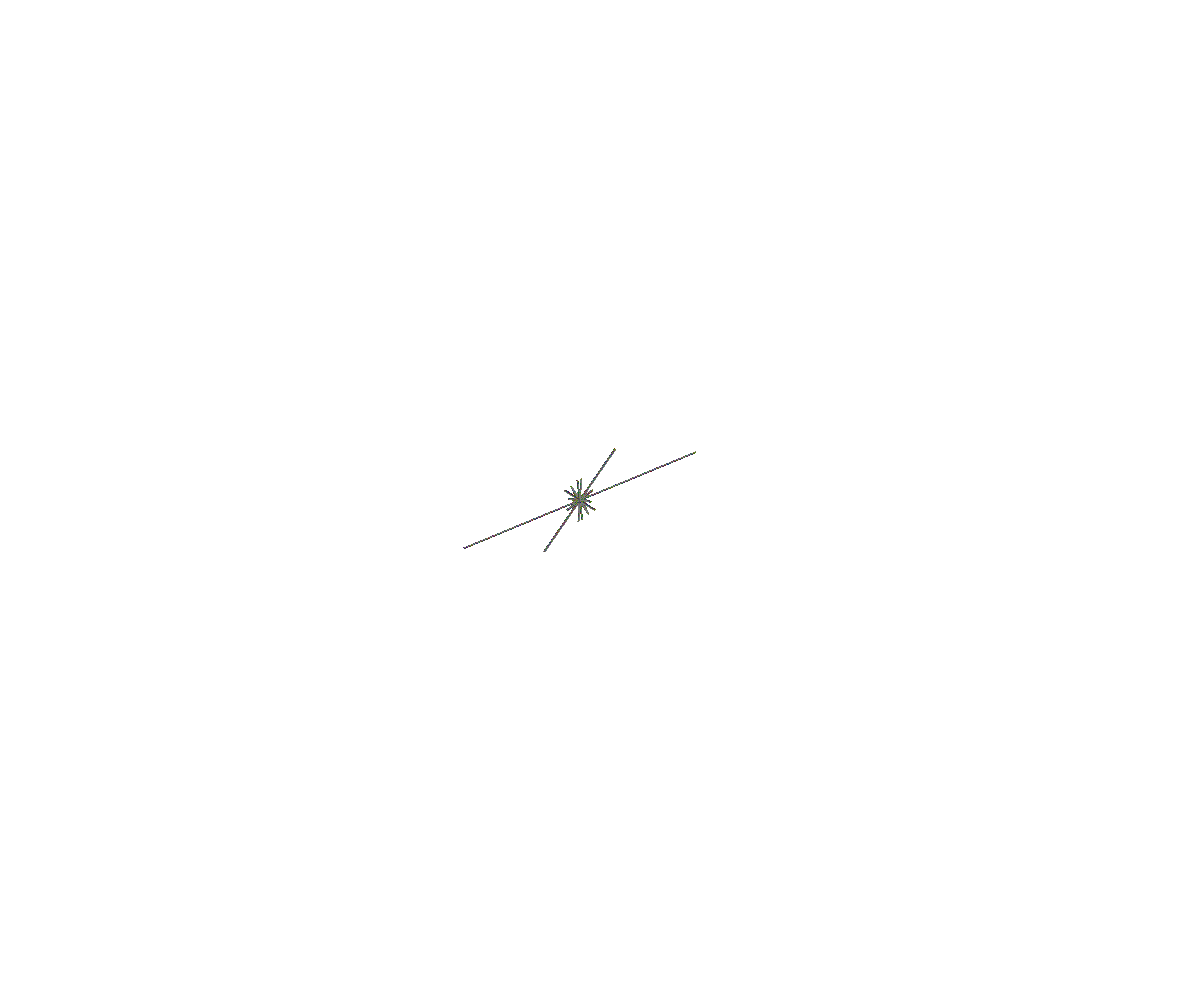
\includegraphics[width=\linewidth]{fig/ecoli_2D.png}
	\label{fig:ecoli_2D}
	\caption{\textit{odgi draw} 2D layout visualization of the 2013 haplotypes E. coli pangenome graph.  
	}
\end{figure*}
	

\end{document}
